%%%%%%%%%%%%%%%%%%%%%%%%%%%%%%%%%%%%%%%%%%%%%%%%%%%%%%%%%%%%%%%%%%%%%%%%%%%%%
%
%  System        : 
%  Module        : 
%  Object Name   : $RCSfile$
%  Revision      : $Revision$
%  Date          : $Date$
%  Author        : $Author$
%  Created By    : Robert Heller
%  Created       : Mon Aug 29 11:04:14 2022
%  Last Modified : <220829.1616>
%
%  Description 
%
%  Notes
%
%  History
% 
%%%%%%%%%%%%%%%%%%%%%%%%%%%%%%%%%%%%%%%%%%%%%%%%%%%%%%%%%%%%%%%%%%%%%%%%%%%%%
%
%    Copyright (C) 2022  Robert Heller D/B/A Deepwoods Software
%			51 Locke Hill Road
%			Wendell, MA 01379-9728
%
%    This program is free software; you can redistribute it and/or modify
%    it under the terms of the GNU General Public License as published by
%    the Free Software Foundation; either version 2 of the License, or
%    (at your option) any later version.
%
%    This program is distributed in the hope that it will be useful,
%    but WITHOUT ANY WARRANTY; without even the implied warranty of
%    MERCHANTABILITY or FITNESS FOR A PARTICULAR PURPOSE.  See the
%    GNU General Public License for more details.
%
%    You should have received a copy of the GNU General Public License
%    along with this program; if not, write to the Free Software
%    Foundation, Inc., 675 Mass Ave, Cambridge, MA 02139, USA.
%
% 
%
%%%%%%%%%%%%%%%%%%%%%%%%%%%%%%%%%%%%%%%%%%%%%%%%%%%%%%%%%%%%%%%%%%%%%%%%%%%%%

\chapter{ESP32-S3-MultiFunction: Multifunction board using an ESP32-S3FN8}

This is a circuit board that is based around an Espressif ESP32-S3FN8 MCU to
manage and operate a collection of model railroad sensors and actuators. The 
board contains these I/O sections:

\begin{itemize}
\item Four occupancy detectors.  CT Coil type sensors, so they won't work with 
DC systems without an AC bias.
\item Four stall-motor drivers with point sense.
\item Four Schmitt Trigger inputs, meant for push buttons.
\item Four Buffered outputs, by default for Panel LEDS, but with drop in 
resistors, can also drive relays or other loads.
\item Sixteen PWM Led drivers.  These are meant to light lamps in signal 
heads.
\end{itemize}

\section{Circuit Description}

\subsection{Section Interconnect}
\begin{figure}[hbpt]\begin{centering}%
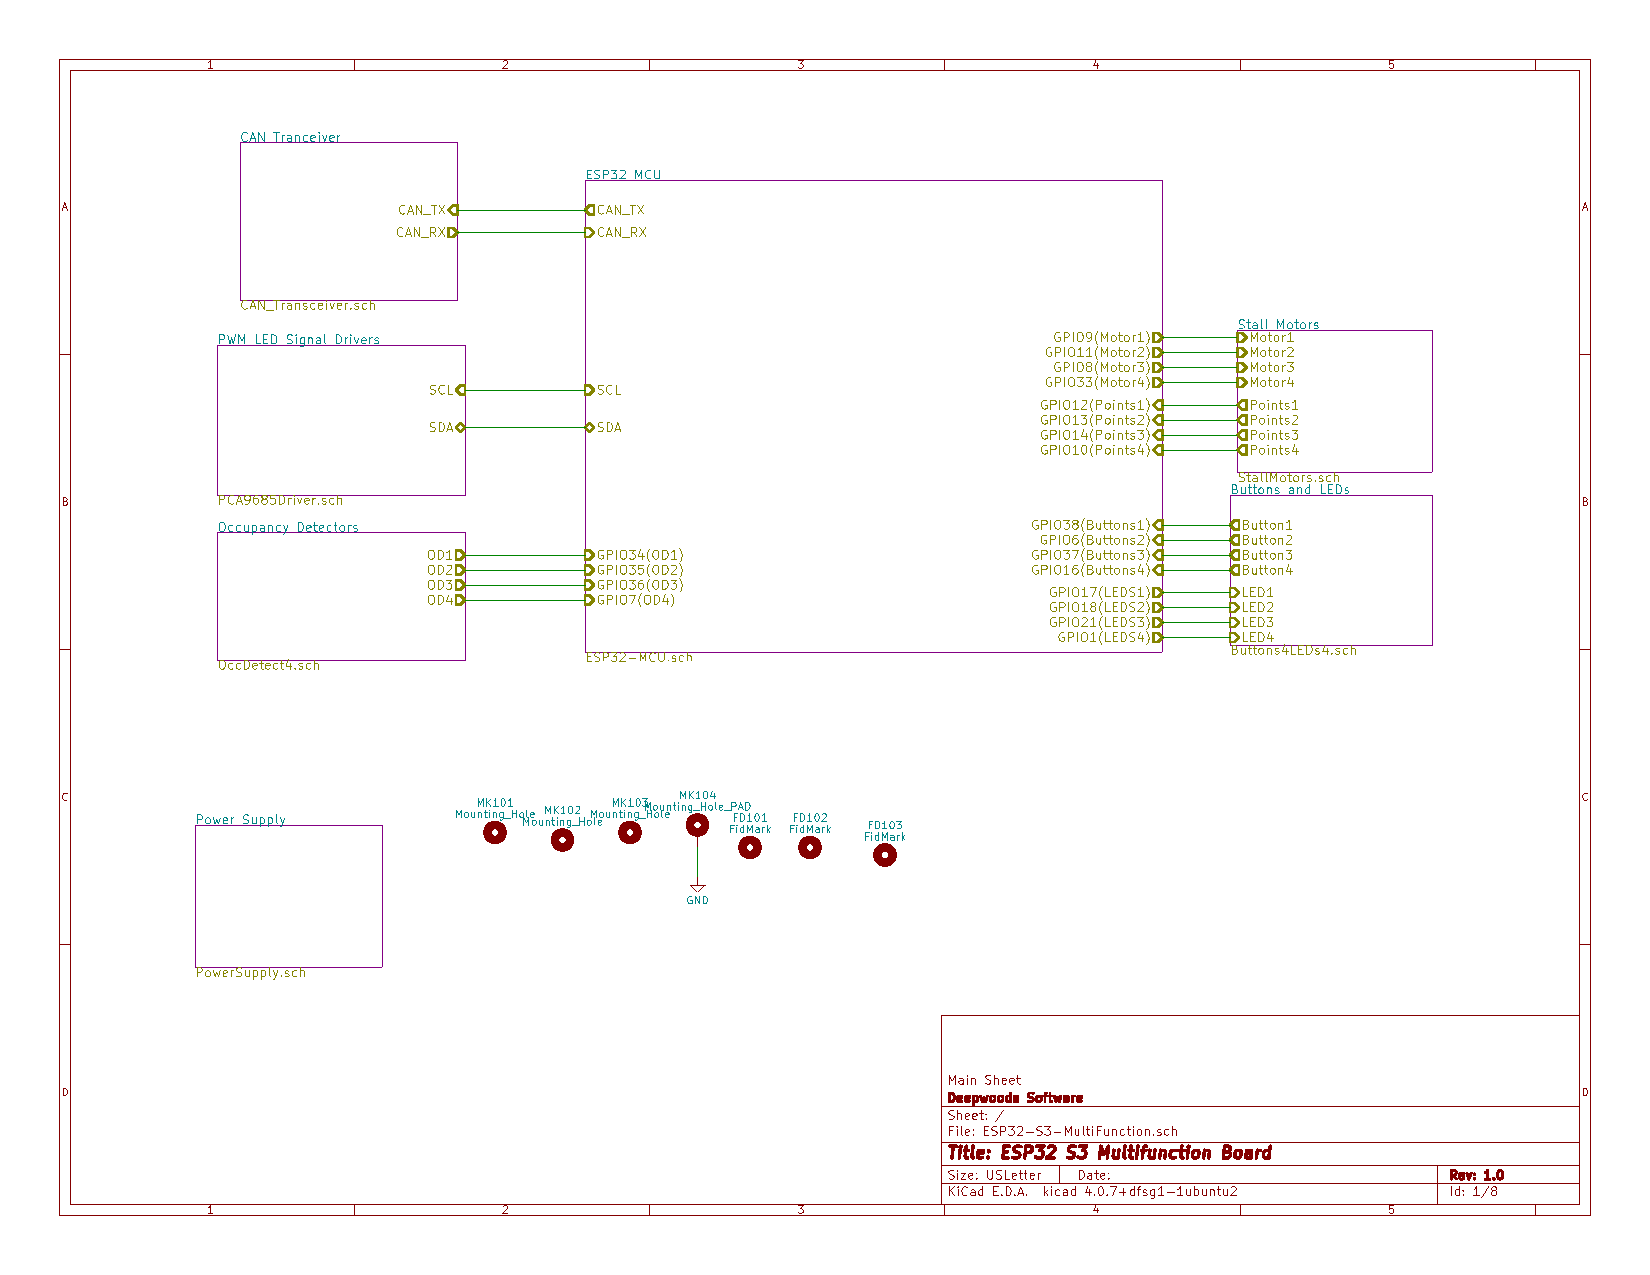
\includegraphics[width=4in]{ESP32-S3-MultiFunction-1.pdf}
\caption{Circuit Diagram of the ESP32-S3-MultiFunction board, page 1: Main 
sheet -- Section Interconnect}
\end{centering}\end{figure}
\begin{figure}[hbpt]\begin{centering}%
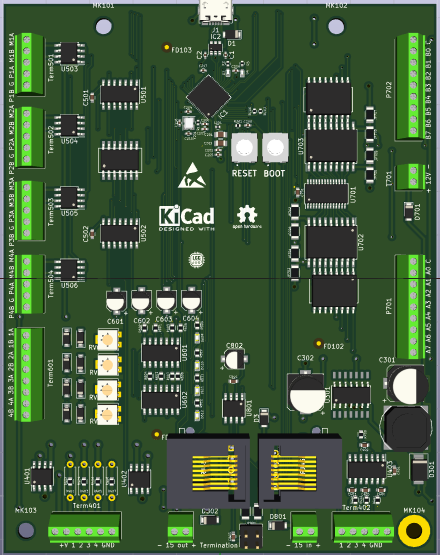
\includegraphics{ESP32-S3-MultiFunction-top3D.png}
\caption{3D Rendering of the whole board.}
\end{centering}\end{figure}

This shows how the various subsections are interconnected.
%\clearpage
\subsection{MCU}
\begin{figure}[hbpt]\begin{centering}%
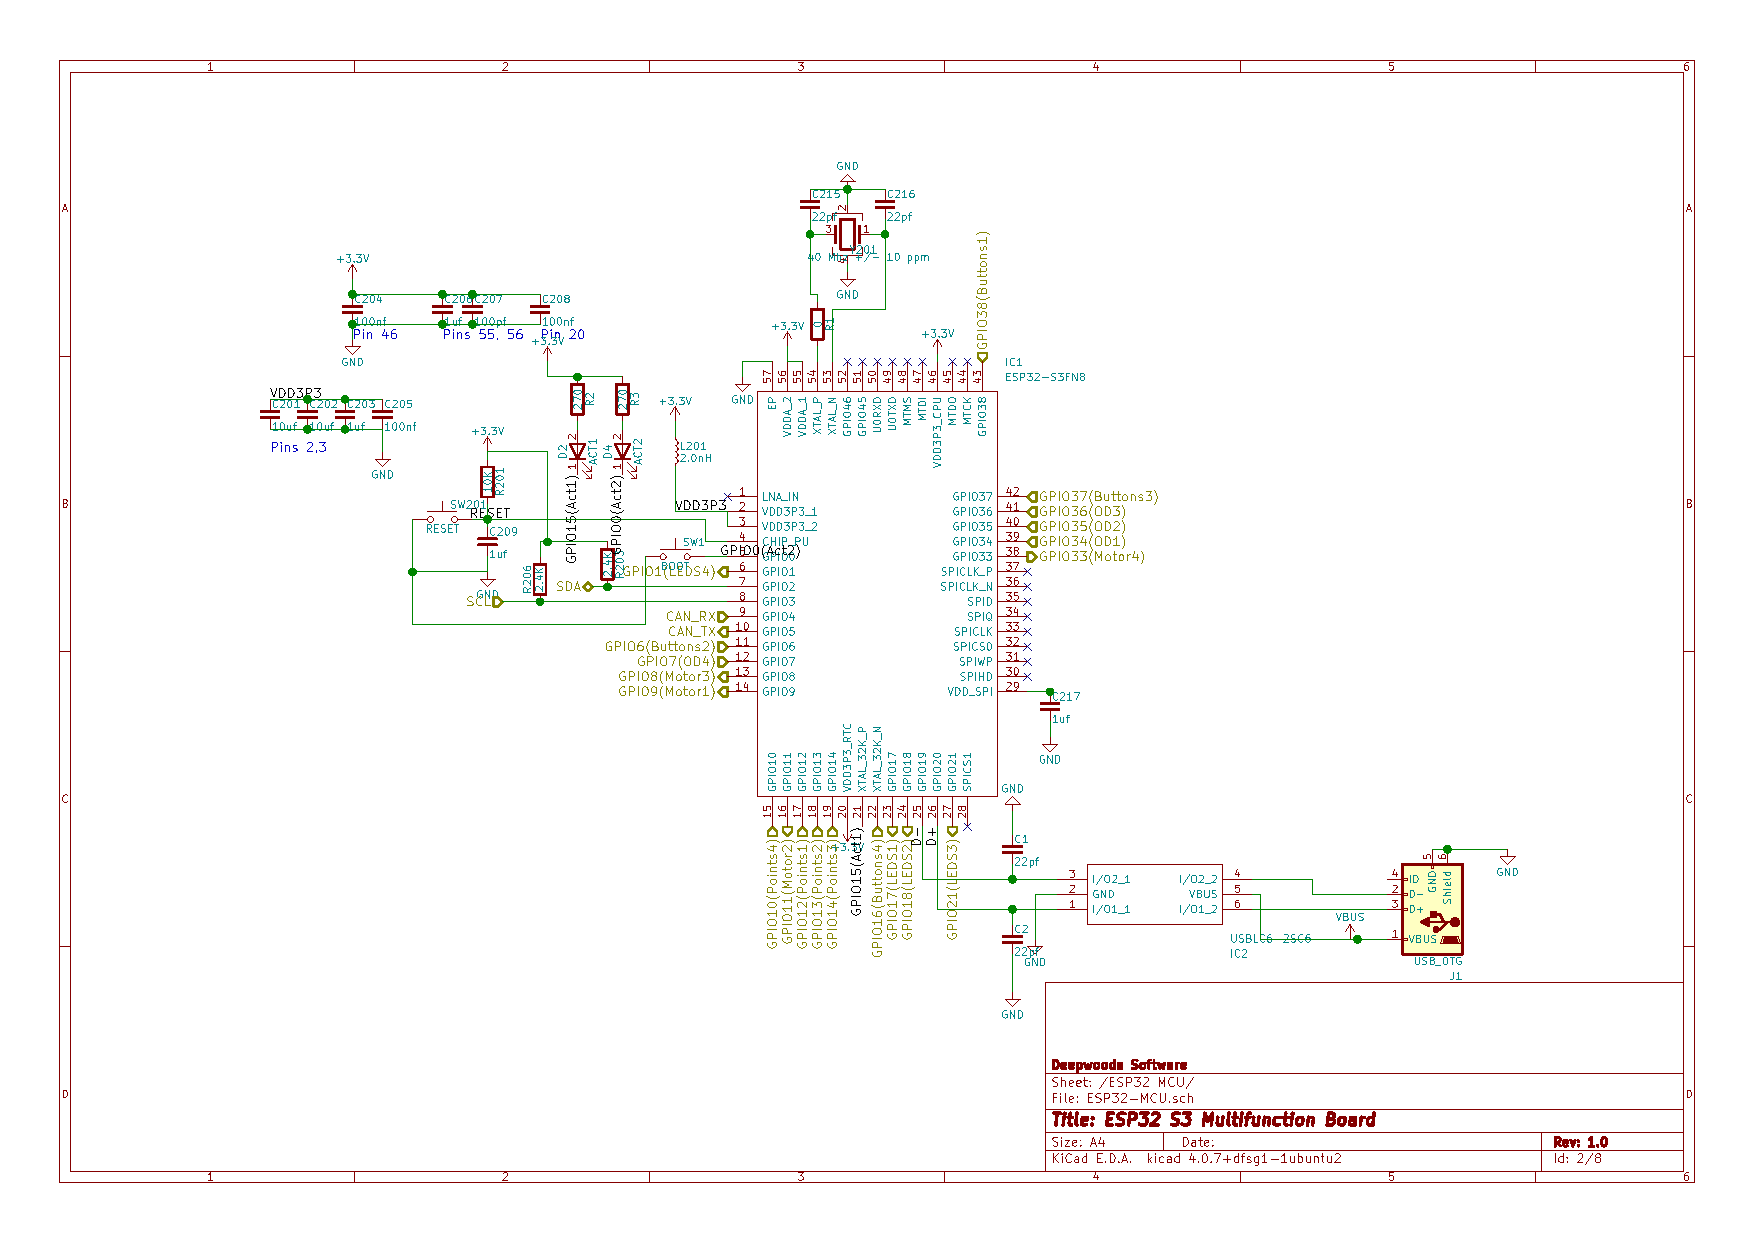
\includegraphics[width=4in]{ESP32-S3-MultiFunction-2.pdf}
\caption{Circuit Diagram of the ESP32-S3-MultiFunction board, page 2: MCU}
\end{centering}\end{figure}
\begin{figure}[hbpt]\begin{centering}%
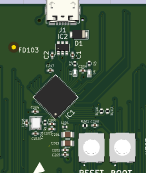
\includegraphics{ESP32-S3-MultiFunction-top3D-MCU.png}
\caption{3D Rendering of the MCU section.}
\end{centering}\end{figure}

This is the MCU and its closely related circuitry, including bypass caps, USB 
connection (for programming and debugging), reset and boot buttons and 
activity LEDS.  There is a micro-B USB connector for programming and 
debugging. 

%\clearpage
\subsection{3.3V Power Supply}
\begin{figure}[hbpt]\begin{centering}%
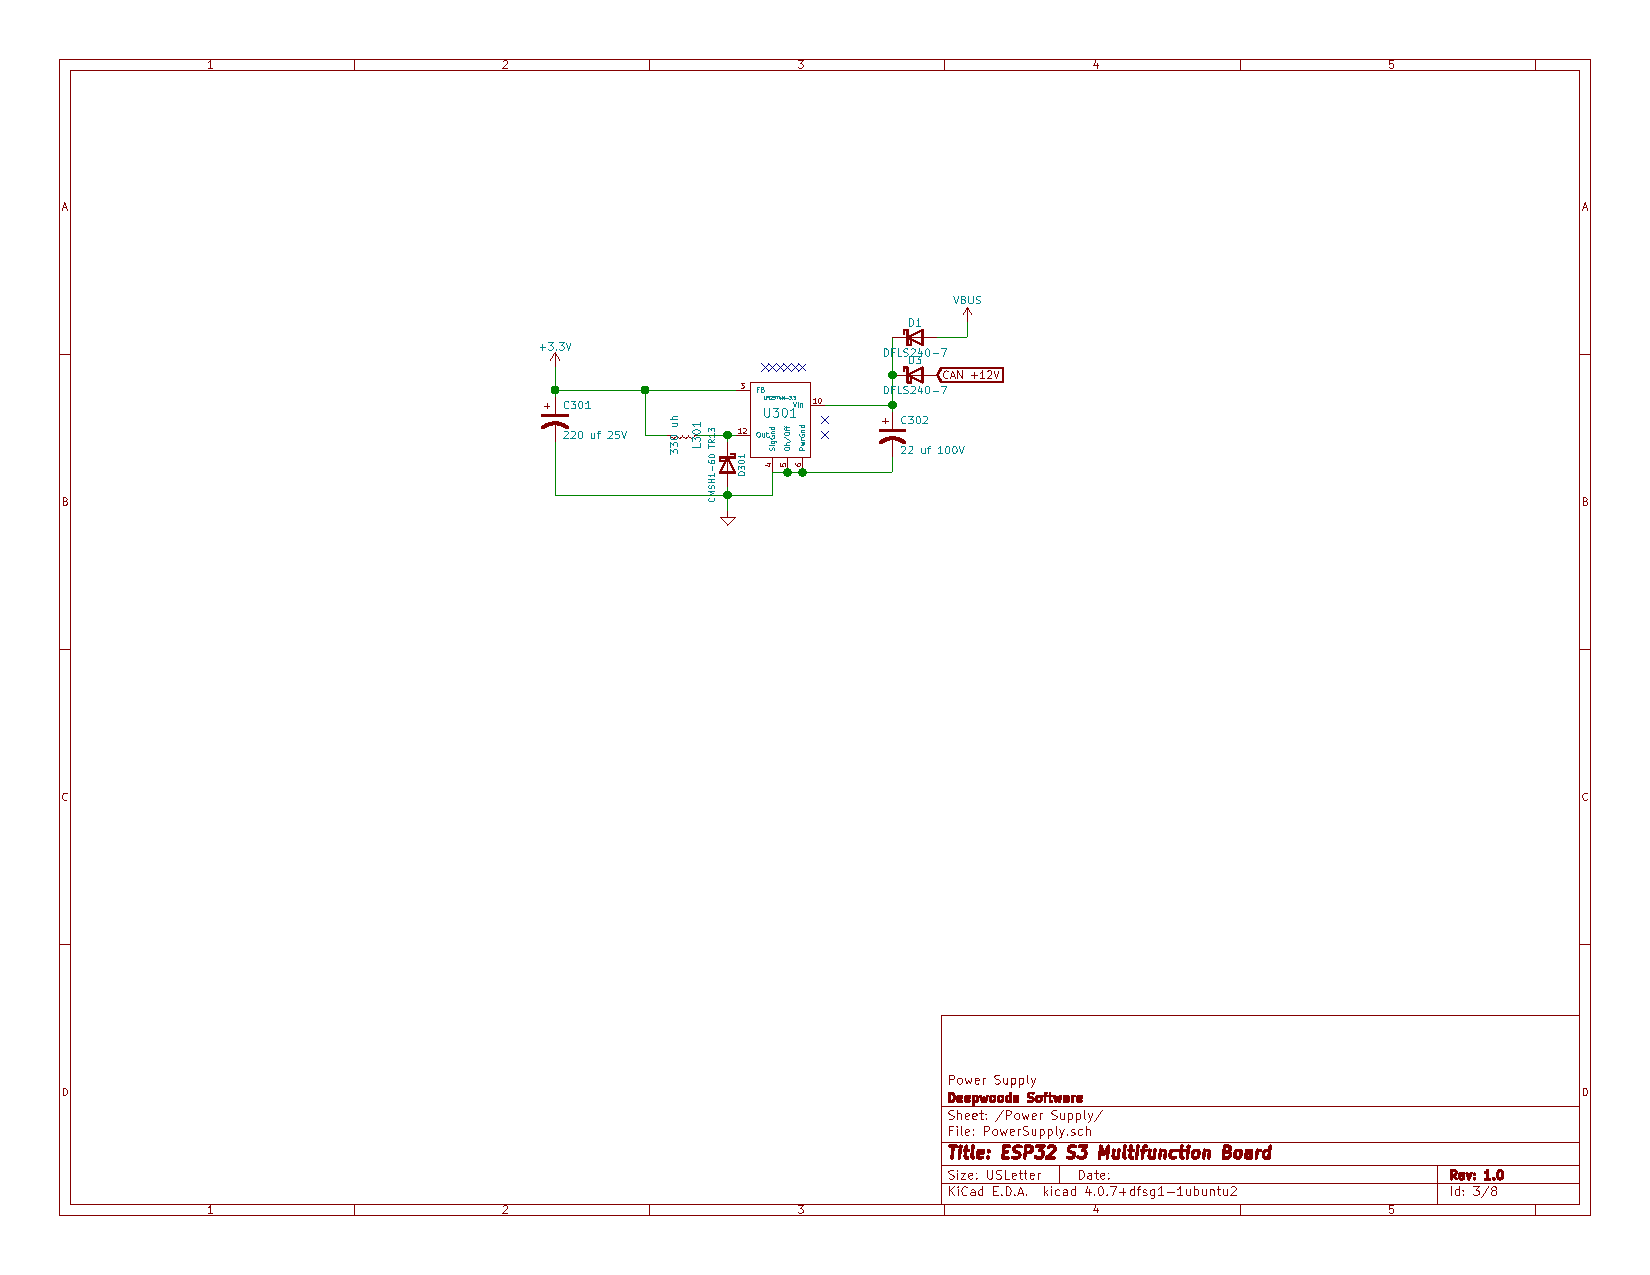
\includegraphics[width=4in]{ESP32-S3-MultiFunction-3.pdf}
\caption{Circuit Diagram of the ESP32-S3-MultiFunction board, page 3: 3.3V 
Power Supply}
\end{centering}\end{figure}
\begin{figure}[hbpt]\begin{centering}%
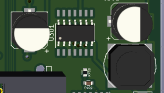
\includegraphics{ESP32-S3-MultiFunction-top3D-PowerSupply.png}
\caption{3D Rendering of the 3.3V Power Supply section.}
\end{centering}\end{figure}

This is the 3.3 volt power supply for all of the logic circuits.

%\clearpage
\subsection{LED Drivers and Buttons}
\begin{figure}[hbpt]\begin{centering}%
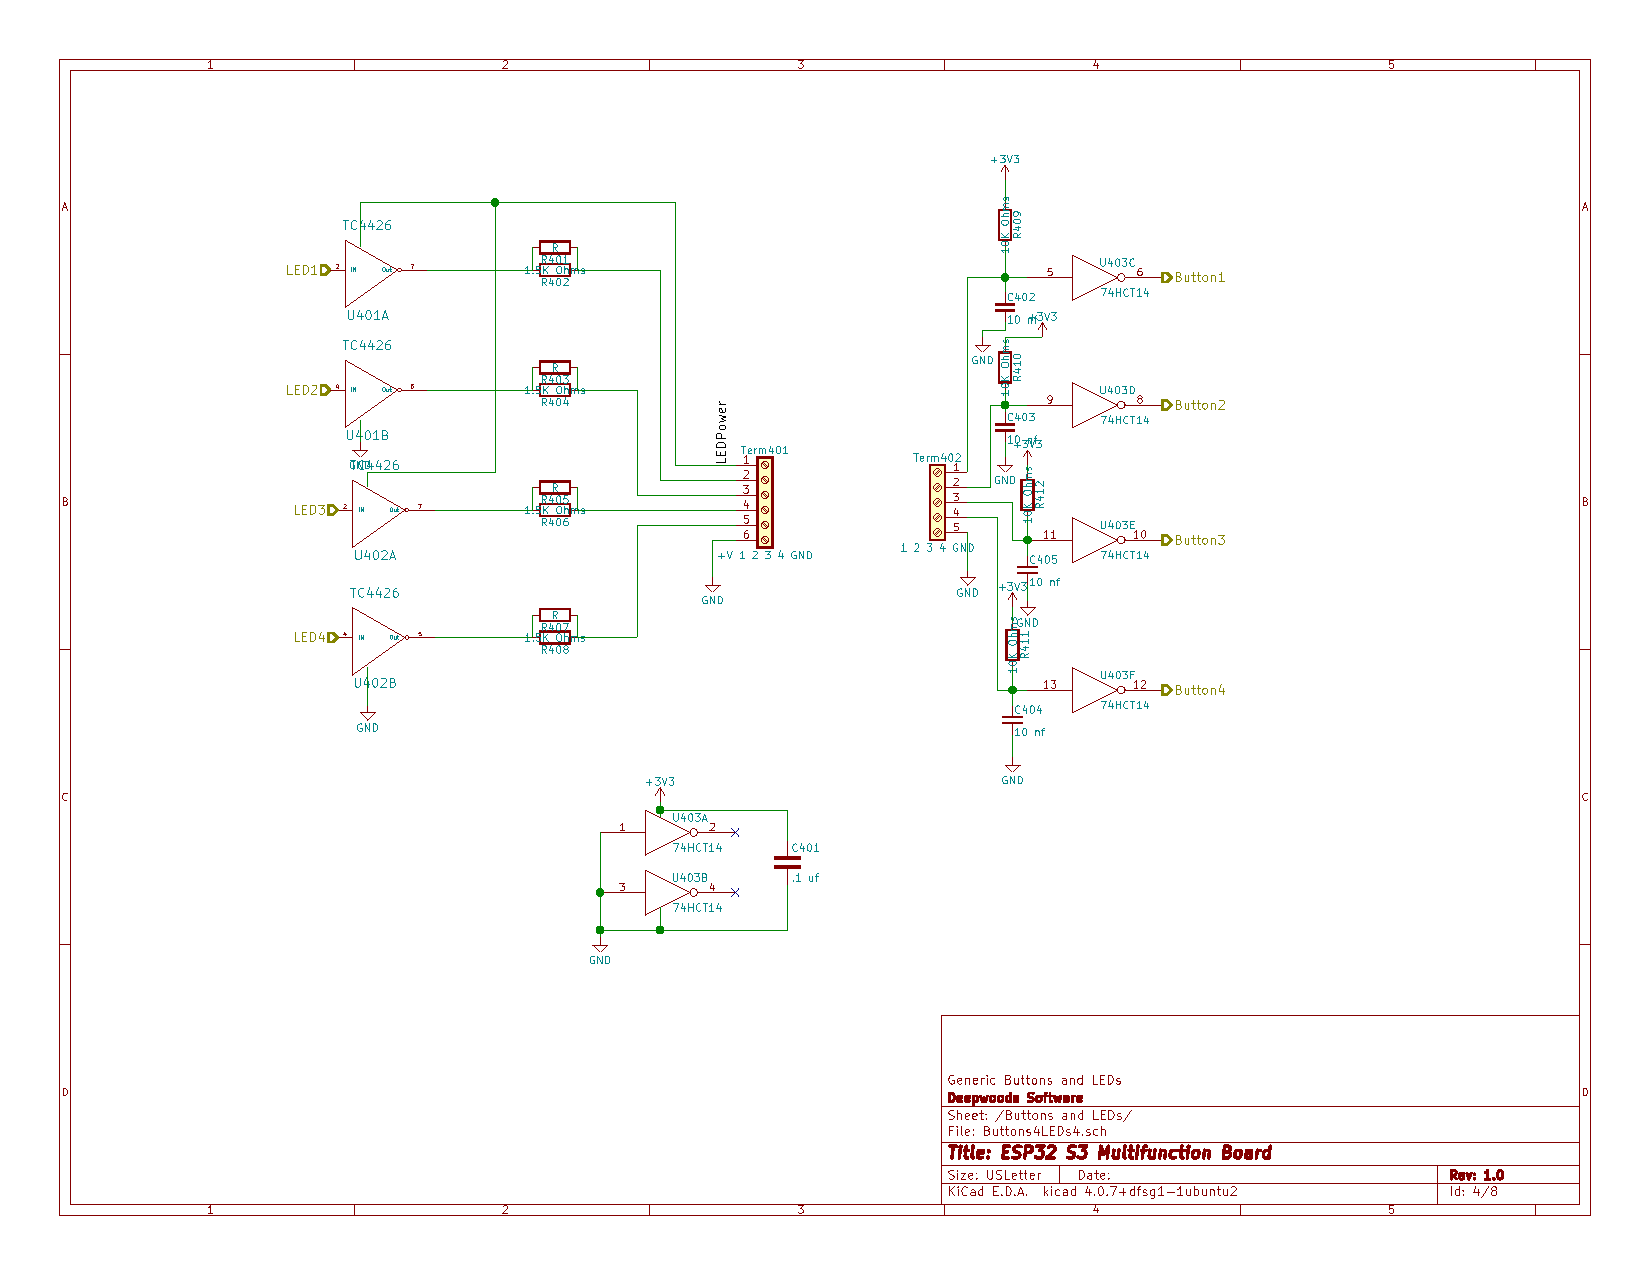
\includegraphics[width=3.5in]{ESP32-S3-MultiFunction-4.pdf}
\caption{Circuit Diagram of the ESP32-S3-MultiFunction board, page 4: LED 
Drivers and Button Inputs}
\end{centering}\end{figure}
\begin{figure}[hbpt]\begin{centering}%
\begin{minipage}{.45\textwidth}
  \centering
  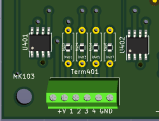
\includegraphics{ESP32-S3-MultiFunction-top3D-LEDDrivers.png}
  \caption{3D Rendering of the LED Drivers Section.}
\end{minipage}
\begin{minipage}{.45\textwidth}
  \centering
  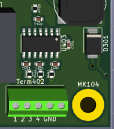
\includegraphics{ESP32-S3-MultiFunction-top3D-Buttons.png}
  \caption{3D Rendering of the Buttons Section.}
\end{minipage}\end{centering}\end{figure}

This is the driver ciruits for the generic LED (or other devices) outputs and
the four push button inputs. The driver outputs have 1.5K Ohm resistors
soldered to the board, which limits the current to about 10ma at 12V and have
places to solder through hole resistors to bypass these resistors to allow for
higher currents (up to 1.5A). The outputs need an external (nomially 12V,
referenced to system ground) supply for these outputs.

The four inputs are buffered with Schmitt Triggers, which provides hardware 
bounce processing.

There is a 6 position (2.54mm pitch) screw terminal for the LED Driver 
outputs.  One end is for the +V (nomially 12V) power source and the other end 
is the ground (-) connection.  In between these terminals are the four 
outputs, which can be driven either high or low.

For the button inputs there is a 5 position (2.54mm pitch) screw terminal 
block. One end is common ground and the other four are for the four buttons.

\subsection{Turnout Control} 
\begin{figure}[hbpt]\begin{centering}%
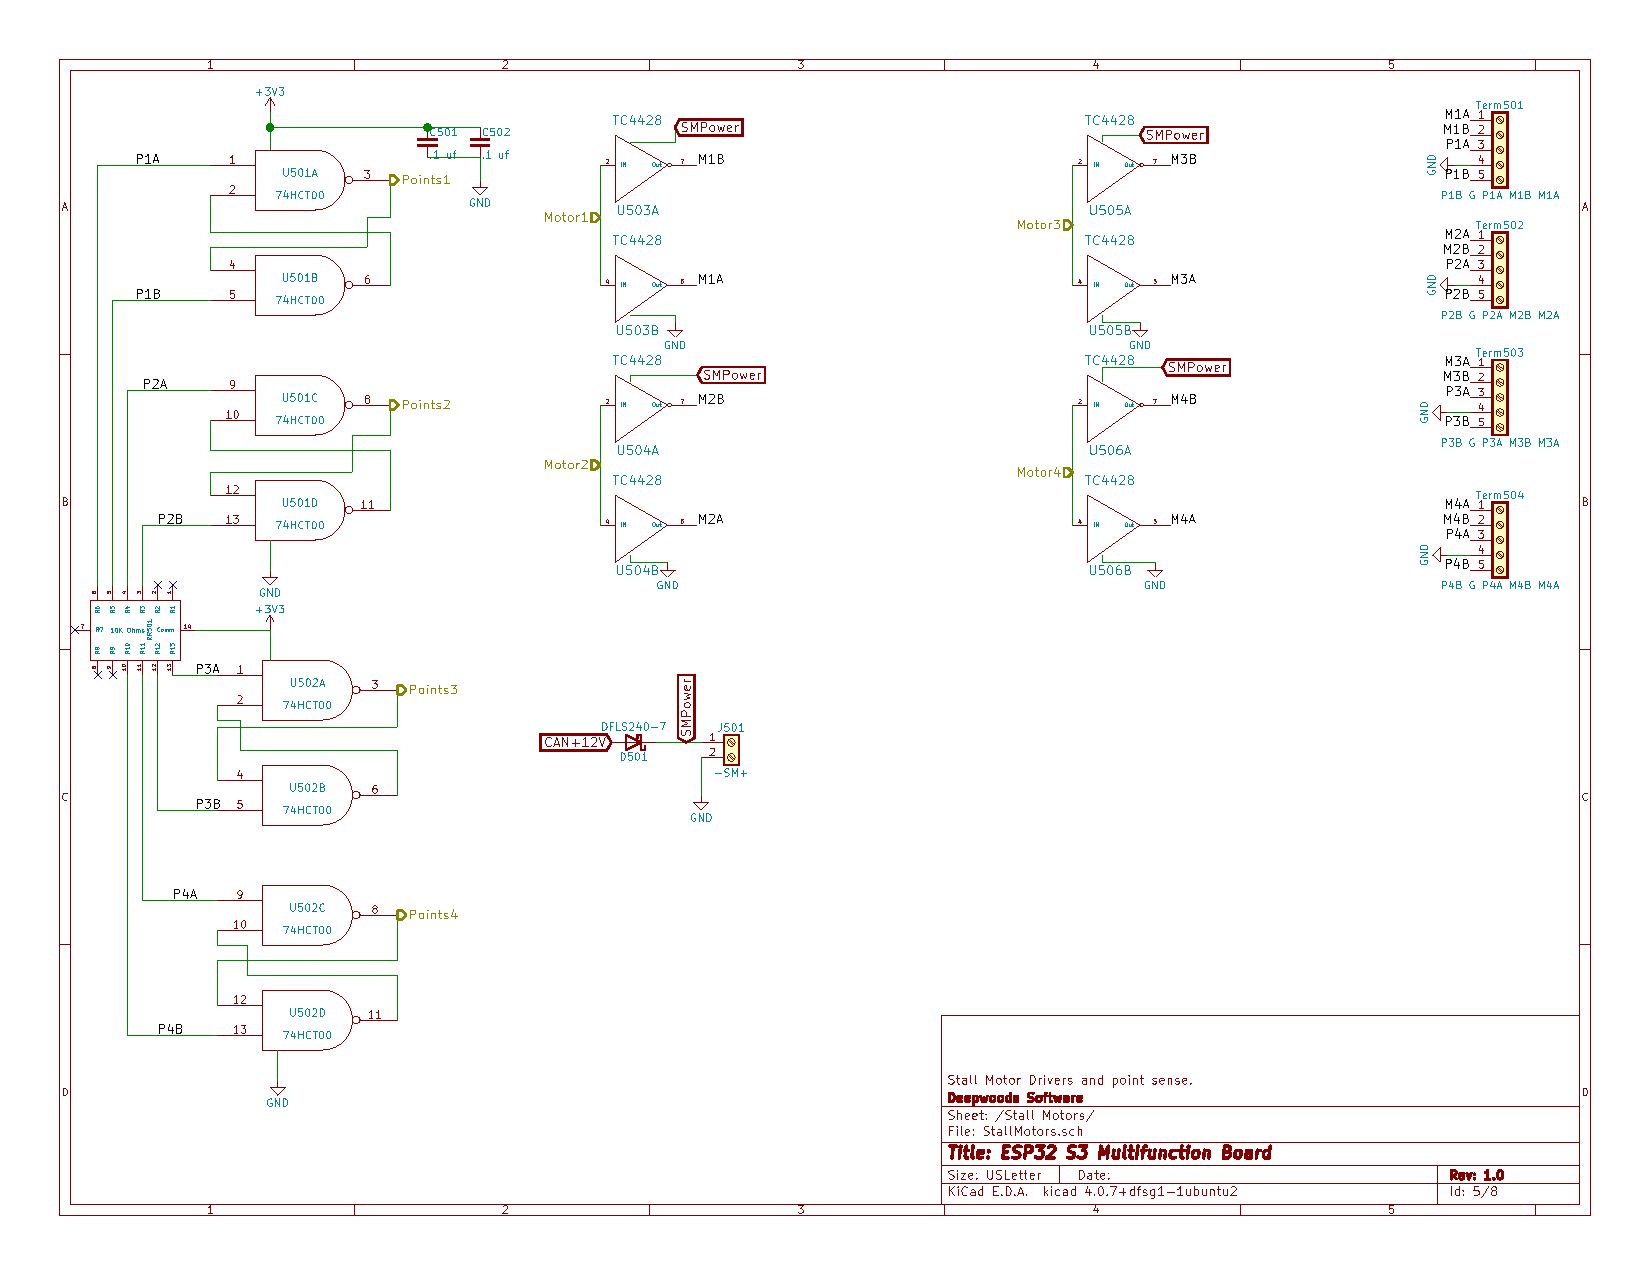
\includegraphics[width=4in]{ESP32-S3-MultiFunction-5.pdf}
\caption{Circuit Diagram of the ESP32-S3-MultiFunction board, page 5: Turnout 
Drivers and Point Sense}
\end{centering}\end{figure}
\begin{figure}[hbpt]\begin{centering}%
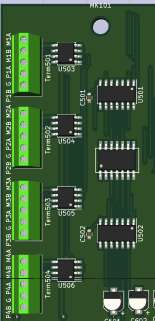
\includegraphics{ESP32-S3-MultiFunction-top3D-Turnouts.png}
\caption{3D Rendering of the Turnouts Section.}
\end{centering}\end{figure}

The Turnout Control section has two parts, a driver part and a sense part.  
For each turnout there is a 5 position (2.54mm pitch) screw terminal block, 
with the connections MA, MB, PA, GND PB.   The MA and MB drive the motor at 
nominally 12 volts.  The PA and PB with the GND connection expect a SPST 
switch mechanically connected to the points (one pole of the internal switch 
in a Tortoise switch motor will work as well).

\clearpage
\subsection{Occupancy Detectors}
\begin{figure}[hbpt]\begin{centering}%
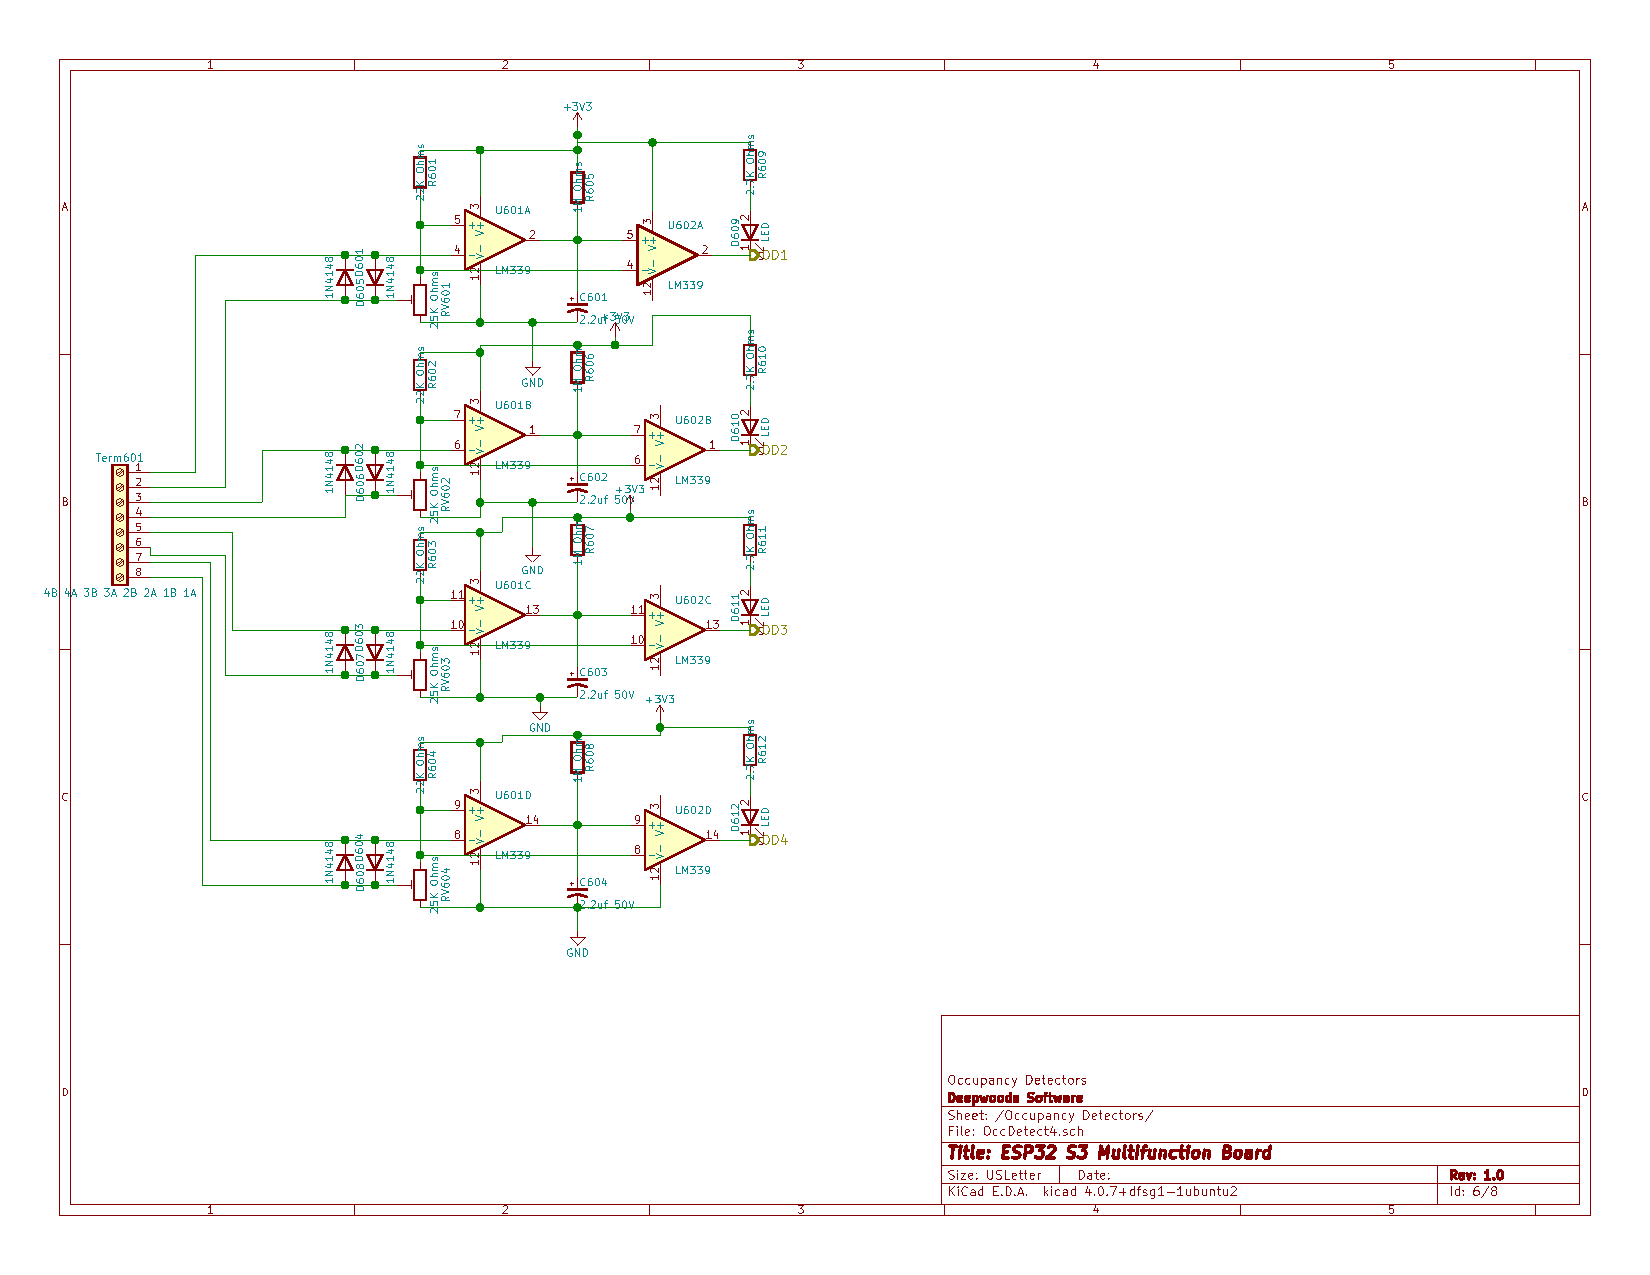
\includegraphics[width=4in]{ESP32-S3-MultiFunction-6.pdf}
\caption{Circuit Diagram of the ESP32-S3-MultiFunction board, page 6: 
Occupancy Detectors}
\end{centering}\end{figure}
\begin{figure}[hbpt]\begin{centering}%
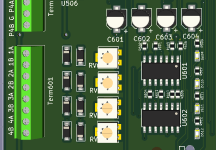
\includegraphics{ESP32-S3-MultiFunction-top3D-OccupancyDetectors.png}
\caption{3D Rendering of the Occupancy Detectors Section.}
\end{centering}\end{figure}

The occupancy detector circuits use a pair of comparitors to detect current in 
a current transformer coil (CT Coil) that would have a track power feeder 
going through it.  The sensitivity can be adjusted and there are indicator 
LEDS on the board.  There is an 8 position (2.54mm pitch) screw terminal 
block, adjacent pairs of terminals are used for each detector.

%\clearpage
\subsection{PWM Signal Lamp drivers}
\begin{figure}[hbpt]\begin{centering}%
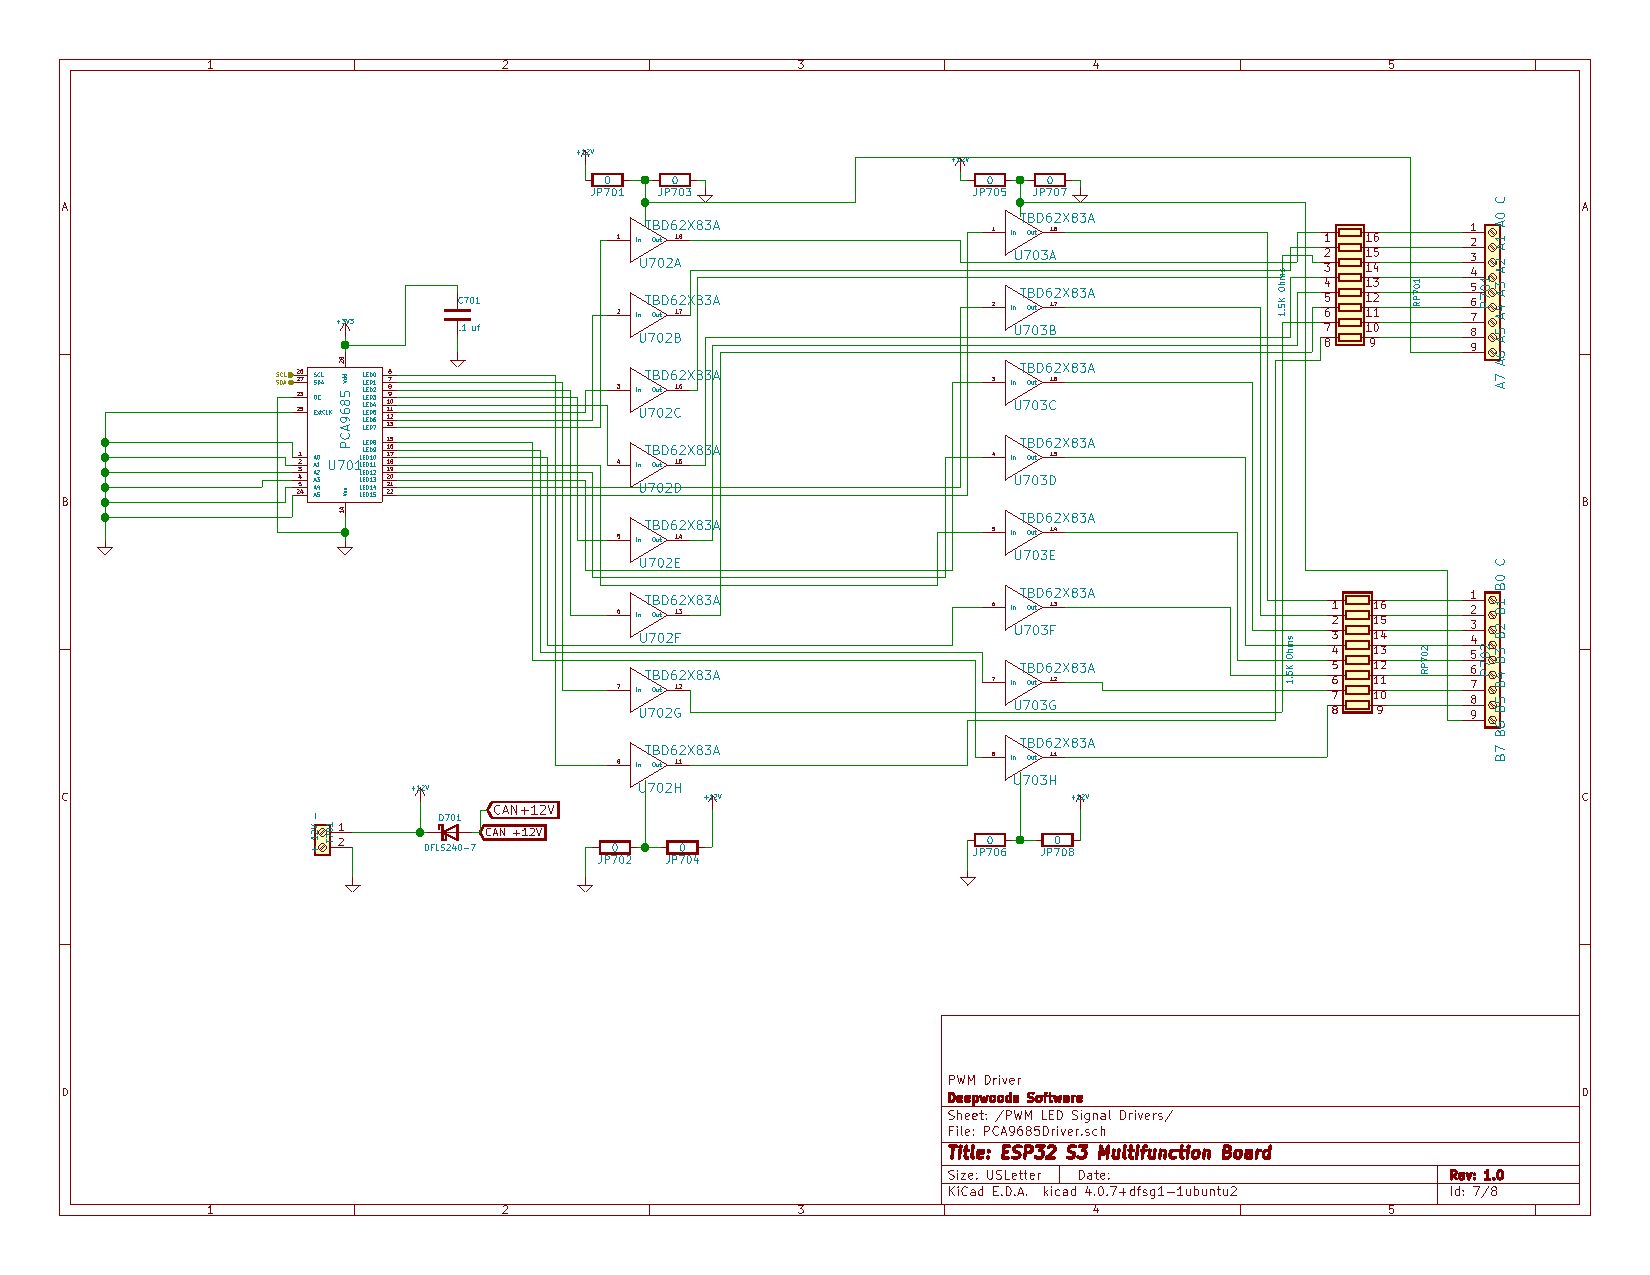
\includegraphics[width=4in]{ESP32-S3-MultiFunction-7.pdf}
\caption{Circuit Diagram of the ESP32-S3-MultiFunction board, page 7: PWM 
Signal Lamp drivers}
\end{centering}\end{figure}
\begin{figure}[hbpt]\begin{centering}%
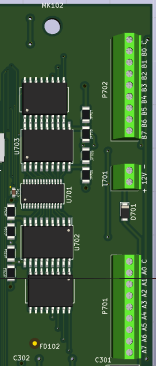
\includegraphics{ESP32-S3-MultiFunction-top3D-PWMSignalLamps.png}
\caption{3D Rendering of the PWM Signal Lamps Section.}
\end{centering}\end{figure}

The PWM Signal Lamp drivers use a PCA9685 which is a 16 channel, 12 bit PWM
LED driver. A pair of octal MOSFET drivers and series load resistors are also
included on the board. The MOSFET drivers come in both inverting (low-side
drive) and non-inverting (high-side drive), so it is possible to support both
common anode and common cathode LED signals. 

There are two 9 position (2.54mm pitch) screw terminal blocks, one for each
bank of 8 lamps (A and B), with a common terminal for each. There is also a 2
position (2.54mm pitch) screw terminal block to optionally provide separate
power for the Signal Lamps.

%\clearpage
\subsection{CAN Transceiver}
\begin{figure}[hbpt]\begin{centering}%
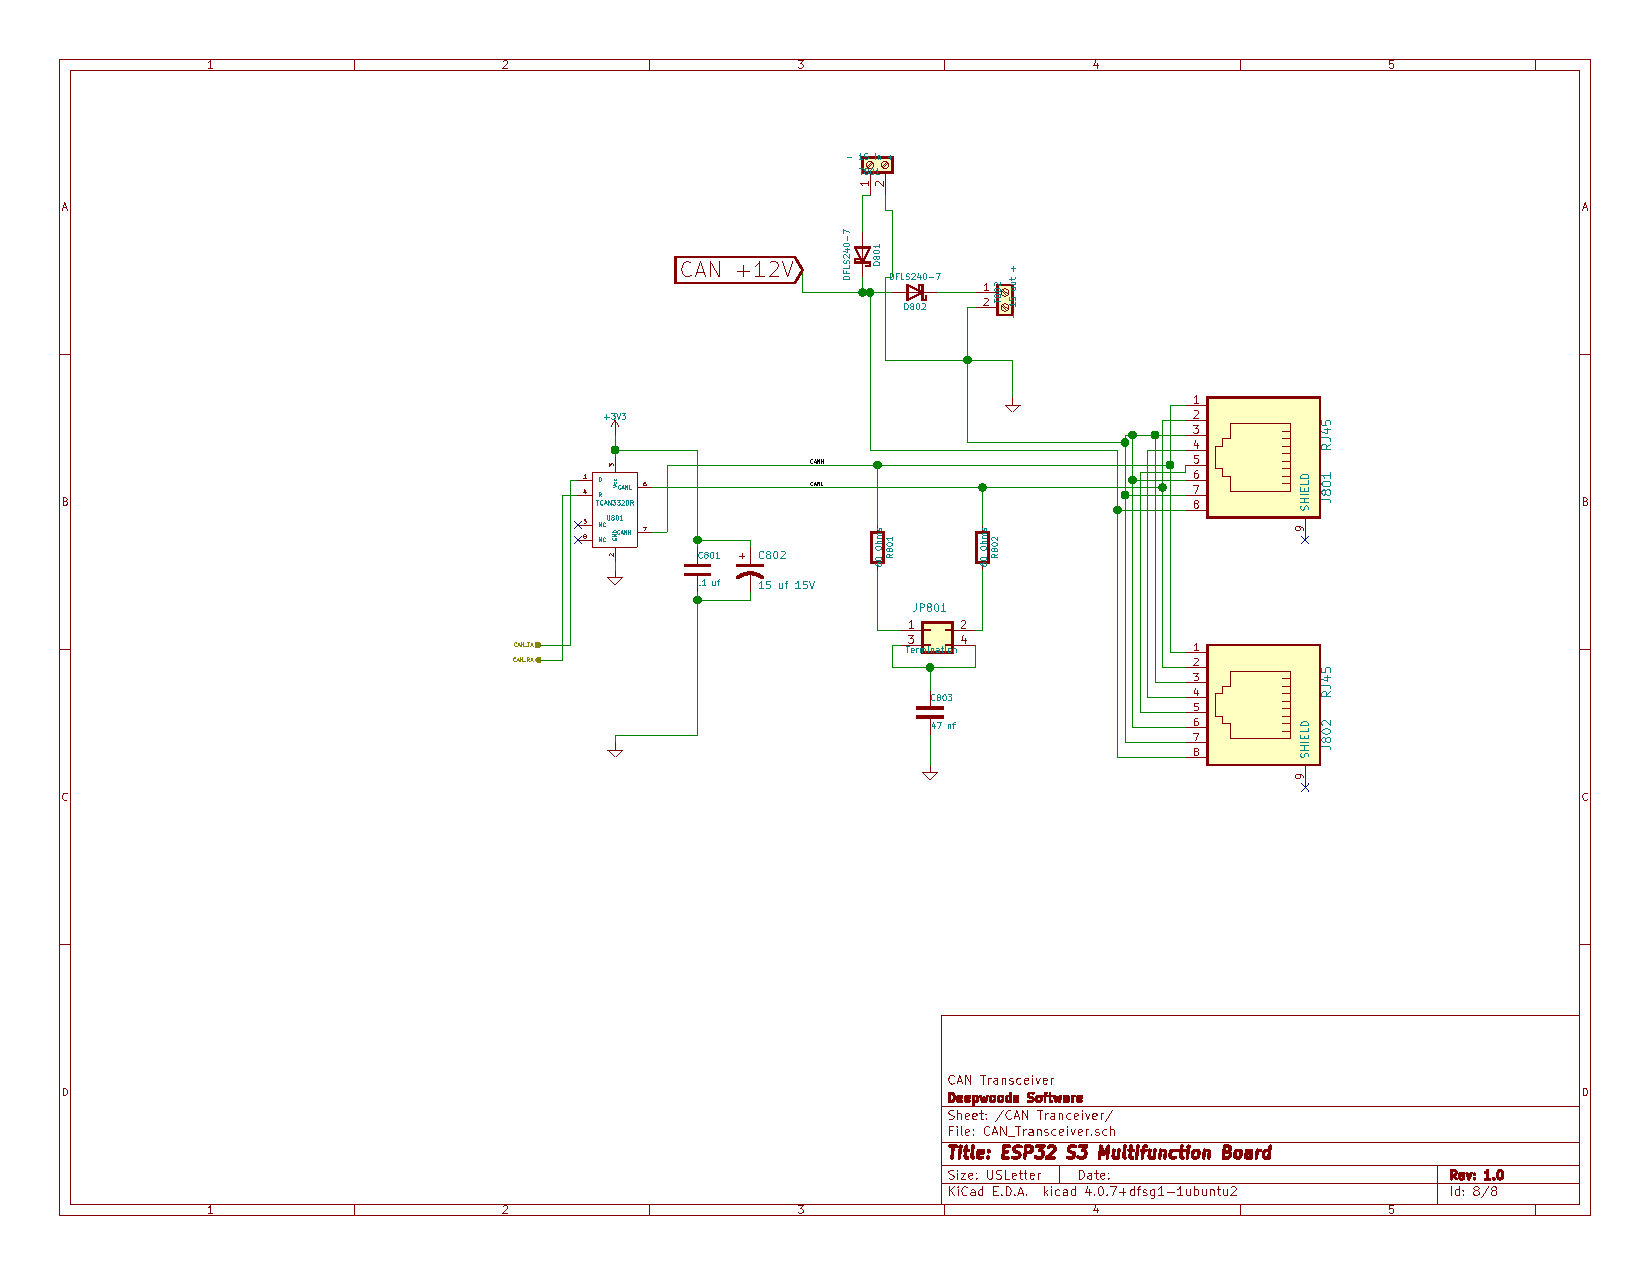
\includegraphics[width=4in]{ESP32-S3-MultiFunction-8.pdf}
\caption{Circuit Diagram of the ESP32-S3-MultiFunction board, page 8: CAN 
Transceiver}
\end{centering}\end{figure}
\begin{figure}[hbpt]\begin{centering}%
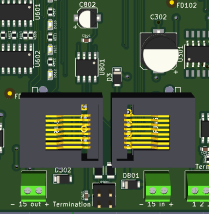
\includegraphics{ESP32-S3-MultiFunction-top3D-CANTransceiver.png}
\caption{3D Rendering of the CAN Transceiver  Section.}
\end{centering}\end{figure}

The CAN Transceiver (TCAN332DR) converts the TTL CAN TX and CAN RX signals to 
CAN\_H and CAN\_L signals and connects them to the pair a parallel wired RJ45 
jacks.  There is also a termination jumper block and 2 position (2.54mm pitch) 
screw terminal blocks to access power in or out of the CAN network.

\clearpage

\section{General Wiring Notes}

There are various terminal blocks, connectors, and jumper blocks on this 
board.  At the bottom edge near the center of the board are a pair of two 
position terminal blocks, one for injecting power into the LCC bus and one for 
extracting power from the LCC bus. Between these terminal blocks is the 
termination jumper block for the LCC bus.  Above the LCC power terminal blocks 
is a pair of RJ45 connectors. These are for connecting the board to the LCC 
bus. These connectors are wired in parallel. Down along the left side 
are the four stall motor terminal blocks (5 position terminal blocks) 
and the occupancy detector terminal block (8 position terminal block).  On the 
lower left edge of the board is a 6 position terminal block for the LED Driver 
outputs and on the lower right edge is a 5 position terminal block for the 
input buttons.  On the right side are two 9 position terminal blocks for the 
signal lamp LEDs. Finally, between the terminal blocks for the signal lamp 
LEDs is a two position terminal block to (optionally) provide power for the 
signal lamp LEDs.

\subsection{LCC Power}

Power can be optionally injected into the LCC bus or extracted from the LCC 
bus. Power can be injected to into the LCC bus to power this and other boards. 
Power can also be extracted to power local devices.

\subsection{LCC Bus connections and termination}

\begin{figure}[hbpt]\begin{centering}%
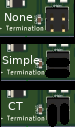
\includegraphics{ESP32-S3-MultiFunction-termination.png}
\caption{Termination Jumper Options}
\label{fig:ESP32-S3-MultiFunction-termination}
\end{centering}\end{figure}
The two RJ45 connections connect to the LCC bus.  If this board is at the end 
of bus, you will need to terminate the bus.  There are two possible 
termination options as shown in 
Figure~\ref{fig:ESP32-S3-MultiFunction-termination}.  With no jumpers 
installed the bus is not terminated, with jumpers installed horizontally 
(parallel to the bottom edge), you will have simple termination (120 Ohms 
across the CAN bus), with jumpers installed vertically, you will have 
center-tap termination (with a 47pf cap to ground).




